
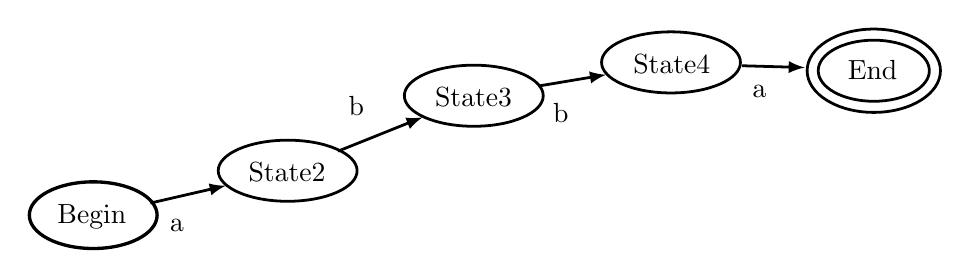
\begin{tikzpicture}[>=latex,line join=bevel,]
  \pgfsetlinewidth{1bp}
%%
\pgfsetcolor{black}
  % Edge: State4 -> End
  \draw [->] (258.55bp,66.794bp) .. controls (262.56bp,66.68bp) and (266.76bp,66.561bp)  .. (281.14bp,66.152bp);
  \definecolor{strokecol}{rgb}{0.0,0.0,0.0};
  \pgfsetstrokecolor{strokecol}
  \draw (264.75bp,57.618bp) node {a};
  % Edge: State2 -> State3
  \draw [->] (113.11bp,36.032bp) .. controls (119.62bp,38.643bp) and (127.11bp,41.642bp)  .. (143.58bp,48.244bp);
  \draw (119.67bp,52.263bp) node {b};
  % Edge: State3 -> State4
  \draw [->] (185.27bp,59.493bp) .. controls (189.79bp,60.246bp) and (194.6bp,61.05bp)  .. (209.61bp,63.558bp);
  \draw (193.32bp,49.67bp) node {b};
  % Edge: Begin -> State2
  \draw [->] (45.581bp,17.354bp) .. controls (50.937bp,18.587bp) and (56.814bp,19.941bp)  .. (72.72bp,23.603bp);
  \draw (55.083bp,9.3119bp) node {a};
  % Node: State3
\begin{scope}
  \definecolor{strokecol}{rgb}{0.0,0.0,0.0};
  \pgfsetstrokecolor{strokecol}
  \draw (162bp,56bp) ellipse (25bp and 11bp);
  \draw (161.91bp,55.589bp) node {State3};
\end{scope}
  % Node: State2
\begin{scope}
  \definecolor{strokecol}{rgb}{0.0,0.0,0.0};
  \pgfsetstrokecolor{strokecol}
  \draw (95bp,29bp) ellipse (25bp and 11bp);
  \draw (94.762bp,28.679bp) node {State2};
\end{scope}
  % Node: Begin
\begin{scope}
  \definecolor{strokecol}{rgb}{0.0,0.0,0.0};
  \pgfsetstrokecolor{strokecol}
  \draw [very thick] (25bp,13bp) ellipse (23bp and 12bp);
  \draw (24.5bp,12.5bp) node {Begin};
\end{scope}
  % Node: End
\begin{scope}
  \definecolor{strokecol}{rgb}{0.0,0.0,0.0};
  \pgfsetstrokecolor{strokecol}
  \draw (306bp,65bp) ellipse (20bp and 11bp);
  \draw (306bp,65bp) ellipse (24bp and 15bp);
  \draw (305.56bp,65.459bp) node {End};
\end{scope}
  % Node: State4
\begin{scope}
  \definecolor{strokecol}{rgb}{0.0,0.0,0.0};
  \pgfsetstrokecolor{strokecol}
  \draw (233bp,68bp) ellipse (25bp and 11bp);
  \draw (233.27bp,67.512bp) node {State4};
\end{scope}
%
\end{tikzpicture}
